\subsection{Comparison of Accuracy vs Noise}

To see how noise affects the accuracy of each method, a number  simulations were
performed, where the noise amplitude on  the  input  step  response function was
continuously increased and the deviation for each method was calculated.

In  the first simulation -- see figure \ref{fig:error_noise_4th}  --  the  input
function was constructed using  a  PT4  element by using Hudzovic's formula with
parameters  $r=0.5$, $n=4$, and  $T=1$.  This  particular  function  was  chosen
because it yielded the most stable results in previous tests.

1000 iterations were performed, starting at 0\% input noise  and  ending at 35\%
input noise. The ever increasing noisy input function was fed into each of the 6
methods. Each method's result was then compared to the original, non-noisy input
function by calculating the root mean squared error.

The resulting error data  was  smoothed  using a sliding average filter of width
10, resulting in figure \ref{fig:error_noise_4th}.

One  issue that arose later with this simulation  was  that  a  systematic  bias
exists  because  all of the calculations are based on a single  input  function.
There  exist a certain combination of time constants $T_k$ that  will  ``align''
better  with  L.  Sani's transfer function (equation \ref{eq:sani}) than with P.
Hudzovic's  transfer  function  (equation   \ref{eq:hudzovic})  and  vica-versa.

In this case, the results in figure \ref{fig:error_noise_4th} happened to use an
input function that favoured P. Hudzovic's method.  This  should be kept in mind
when interpreting the data.

In an effort to eliminate this bias, the simulation was repeated 500 times and a
random  input  function  was generated using equation \ref{eq:random_ptn}.  This
way, no single  method  was favoured. The 500 resulting errors were averaged and
can be seen in figure \ref{fig:error_noise_random}.

Due  to  the  intensive nature of this  simulation,  the  fitting  methods  were
omitted,  because they took too long to compute. It is fairly  certain,  though,
that they would perform better than the other methods.

Finally,by using the same  PT4  element  from  the  first simulation as an input
function, the third simulation  covers an input noise range of 0\% to 200\%. The
results     of     this     simulation     are     visualised      in     figure
\ref{fig:error_noise_long_term}.

\begin{figure}
    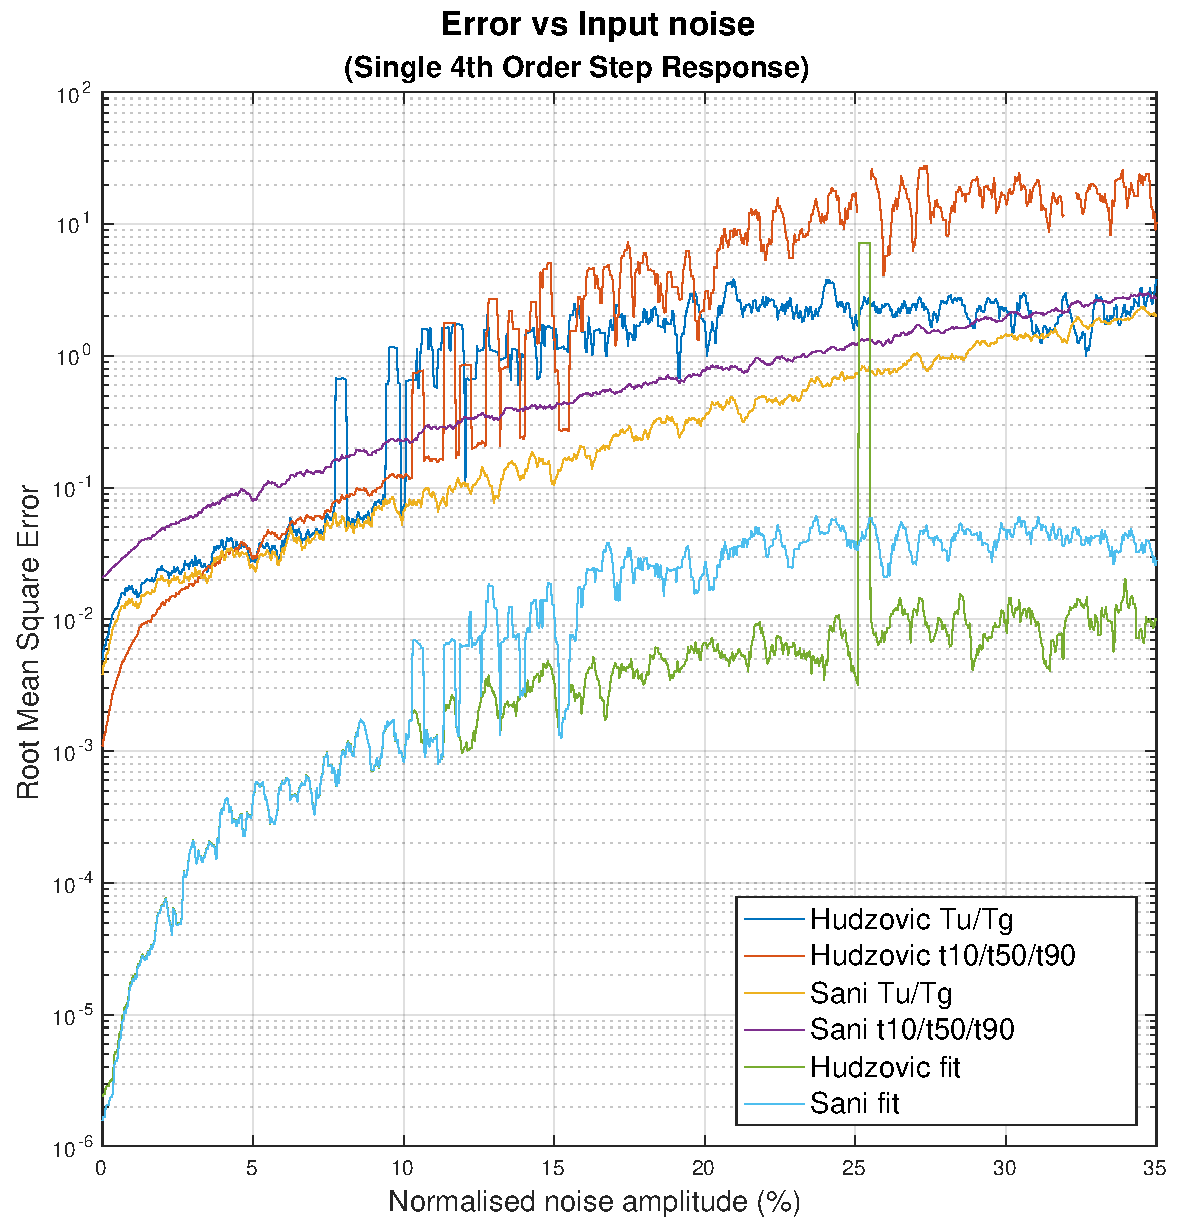
\includegraphics[width=\linewidth]{images/error_noise_4th_order_steps}
    \caption{The root mean square error (RMSE) of each method to the original 4th order step response function, in function of normalised input noise amplitude.}
    \label{fig:error_noise_4th}
\end{figure}
\begin{figure}
    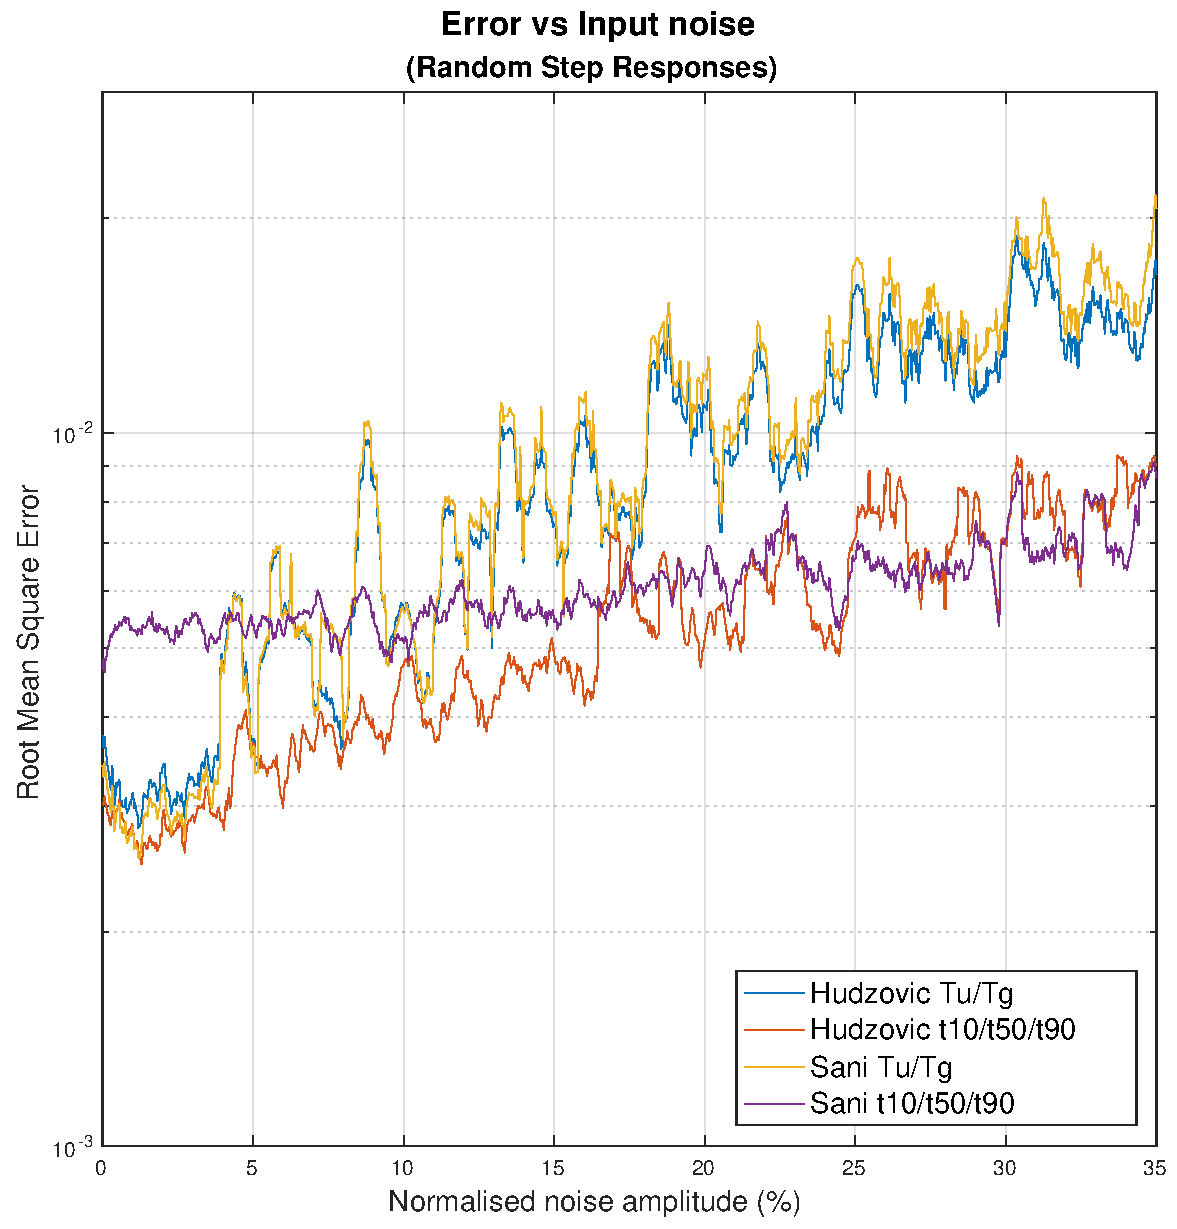
\includegraphics[width=\linewidth]{images/error_noise_random_steps}
    \caption{The root mean square error (RMSE) of each method to a randomly generated nth order step response function, in function of normalised input noise amplitude. The fitted curves were omitted due to their time consuming nature.}
    \label{fig:error_noise_random}
\end{figure}
\begin{figure}
    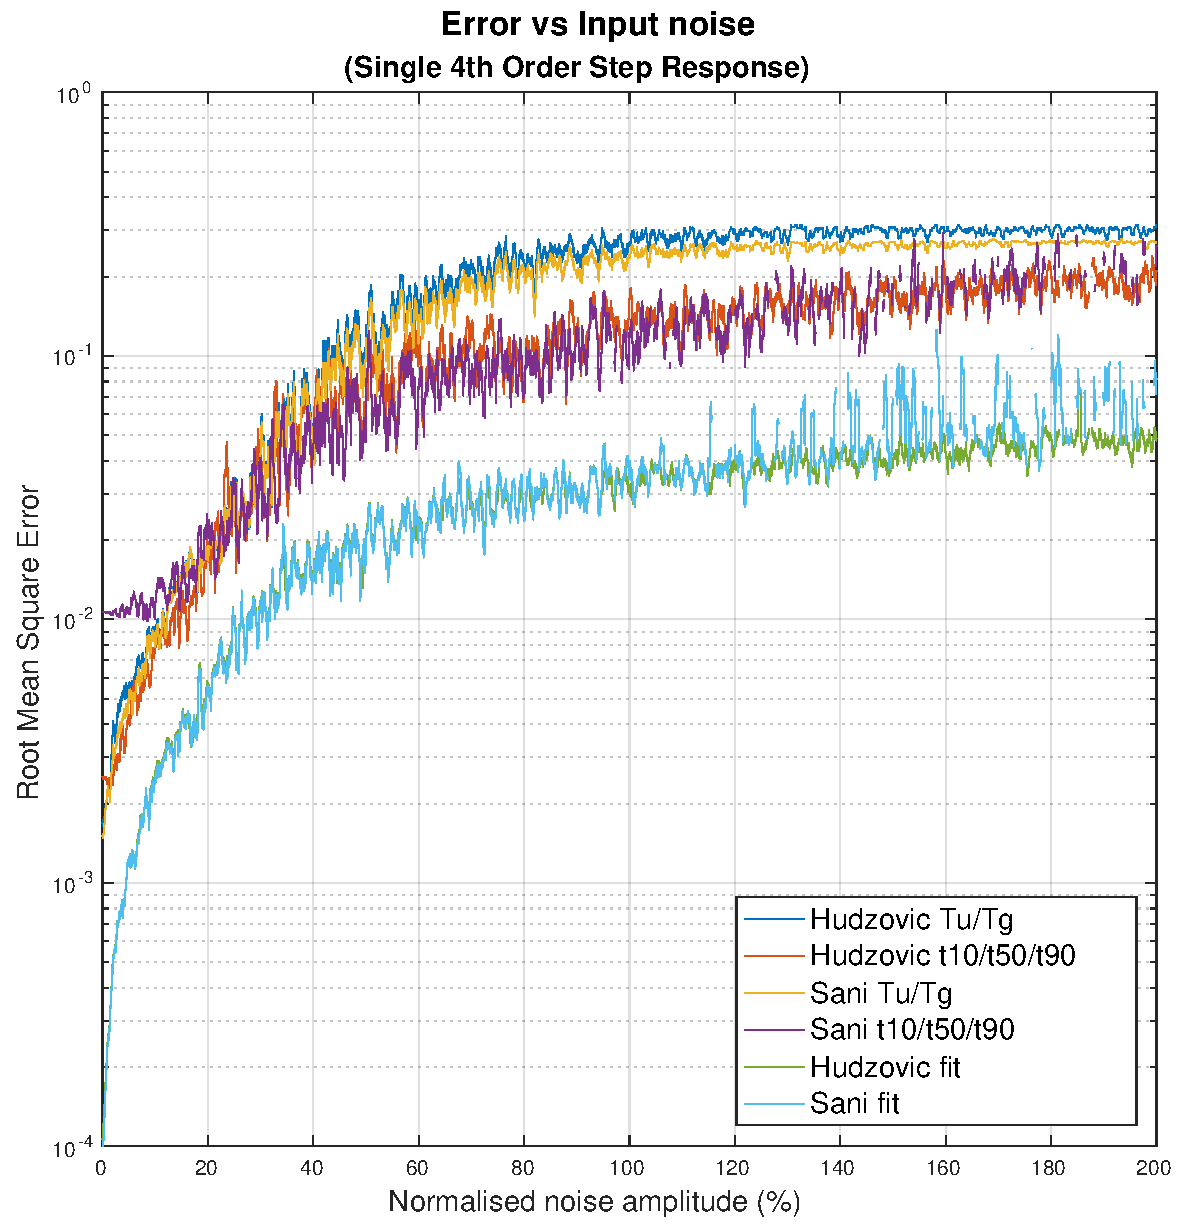
\includegraphics[width=\linewidth]{images/error_noise_long_term}
    \caption{Long term view of the root mean square error (RMSE) of each method to the original 4th order step response function, in function of normalised input noise amplitude.}
    \label{fig:error_noise_long_term}
\end{figure}


\subsubsection*{Conclusions}

An immediate conclusion to be drawn  is  that  the two fitting methods (cyan and
olive  curves  in  figure \ref{fig:error_noise_4th}) yield more accurate results
than any of the other methods by an order of magnitude. This is  to be expected,
of course.  While the Sani fit proves to be the most accurate fitting method for
non-noisy signals, as can be seen by zooming into the bottom left  of  the plot,
the Hudzovic fit proves itself to be the most  accurate  for very noisy signals.

Also as expected,  the  accuracy of each method appears to get less accurate the
more noisy the input signal is.

As  already  mentioned,  the data in figure \ref{fig:error_noise_4th} should  be
interpreted with caution, due to a  systematic  bias.  With  this  in  mind,  an
unexpected  result  in   figure  \ref{fig:error_noise_4th}  is  that  Hudzovic's
characterisation approach using $T_u/T_g$ shows to  be  more  accurate for noisy
signals  than  Sani's  characterisation  approach  using   $t_{10}$,   $t_{50}$,
$t_{90}$. This can be observed by comparing  the  (orange) and (blue) curves, or
by comparing the (purple) and (yellow) curves. This result is unexpected because
of how $T_u/T_g$ is calculated: The derivative of the signal must be computed in
order to find the point of  inflection (see theory section). The derivative of a
noisy signal is, of course, an even noisier signal, which  should make correctly
calculating  the  point  of  inflection much less accurate than calculating  the
threshold values $t_{10}$, $t_{50}$, $t_{90}$.

However,  the  data   in   figure  \ref{fig:error_noise_random}  and  in  figure
\ref{fig:error_order}  directly  contradicts  this  conclusion.  When taking the
average of lots  of  simulations  using random input step response functions, it
appears that the methods using the $T_u/T_g$ characterisation perform worse than
those using $t_{10}$, $t_{50}$, $t_{90}$. This  can especially be seen in figure
\ref{fig:error_noise_random}. At around  4\%  noise amplitude, both methods that
use  the   $T_u/T_g$   characterisation   start   jumping   around   eratically.

The  most  accurate  non-fitting  method  is  Hudzovic's  transfer  function  in
combination  with Sani's characterisation method, $t_{10}$, $t_{50}$,  $t_{90}$.
This appears to be the case in both simulations.
